% ch06 Interacting electron gas (书页 37–50 / 分册p051–p064)
% 第6章 Interacting electron gas
\chapter{相互作用电子气}

现在我们转向讨论金属中相互作用电子的性质。作为第一级近似，我们把离子仅仅视为一团均匀的正电荷背景，用来补偿电子的总电荷。这一近似构成了胶冻模型（Jellium model），它由赫林（Herring）首先引入，并经Pines（P1955）作了广泛的表征。对电荷为$Z$、密度为$n_{\mathrm{i}}$的离子而言，电子密度$n_{\mathrm{e}}$等于$Zn_{\mathrm{i}}$。我们先考虑均匀相互作用电子系统的哈特里–福克近似，它适用于高密度情形；随后再引入进一步的近似来处理相互作用电子气的稀薄区域。

通常，我们把本征态
\begin{equation*}
\phi_{\mathbf{p}}(\mathbf{r}) = \frac{\mathrm{e}^{\mathrm{i}\mathbf{p}\cdot\mathbf{r}/\hbar}}{\sqrt{V}}
\tag{6.1}
\end{equation*}
与在体积为$V$的盒子中、具有周期性边界条件的自由电子相联系。事实表明，这样的自由粒子态也满足电子气胶冻模型的哈特里–福克方程。然而，正如下文所推导的，相应的单粒子能量不再是$p^2/2m$，而是
\begin{equation*}
\epsilon(\mathbf{p}) = \frac{p^2}{2m} - \frac{e^2 p_{\mathrm{F}}}{\pi\hbar}\left(1 + \frac{p_{\mathrm{F}}^2 - p^2}{2pp_{\mathrm{F}}}\ln\left|\frac{p + p_{\mathrm{F}}}{p - p_{\mathrm{F}}}\right|\right).
\tag{6.2}
\end{equation*}

由于电子间的交换关联，同自旋的粒子不会彼此重叠，被占据能级的能量被压低到自由粒子结果之下。因此，哈特里–福克近似给出一种具有确定动量的缀饰（dressed）电子激发。这类激发由平面波本征态描述，这一事实表明，哈特里–福克近似实质上是对电子气的一种无相互作用处理。确实如此：哈特里–福克给出一组试图模仿相互作用系统的无相互作用准粒子。然而我们将会看到，它们对原系统性质的模仿并不成功。例如，哈特里–福克处理无法再现热容随温度的线性依赖，反而预言比热按$\ln T$发散。

\section{均匀电子气}

分析相互作用电子气的出发点是哈特里–福克方程
\begin{equation*}
\begin{aligned}
\epsilon_\nu \phi_\nu(\mathbf{r}) ={} & \left[\frac{-\hbar^2}{2m}\nabla_r^2 + V_{\mathrm{ion}}(r) + e^2\sum_\lambda \int \mathrm{d}\mathbf{r}'\, n_{\phi_\lambda}(r')\frac{1}{|\mathbf{r} - \mathbf{r}'|}\right]\phi_\nu(\mathbf{r}) \\
& - e^2\sum_\lambda \int \mathrm{d}\mathbf{r}'\, \phi_\nu(\mathbf{r}')\phi_\lambda^*(\mathbf{r}')\phi_\lambda(\mathbf{r})\frac{1}{|\mathbf{r} - \mathbf{r}'|}.
\end{aligned}
\tag{6.3}
\end{equation*}
一开始就假定形如式 (6.1) 的平面波态满足哈特里–福克方程，把对动量的求和换成积分，并在交换项中把积分变量变换为$\mathbf{x} = \mathbf{r}' - \mathbf{r}$，我们得到本征值方程
\begin{equation*}
\begin{aligned}
\epsilon(\mathbf{p})\phi_{\mathbf{p}}(\mathbf{r}) ={} & \left[\frac{p^2}{2m} + V_{\mathrm{ion}}(r) + e^2 n_{\mathrm{e}}\int \mathrm{d}\mathbf{r}'\, \frac{1}{|\mathbf{r} - \mathbf{r}'|}\right]\phi_{\mathbf{p}}(\mathbf{r}) \\
& - e^2\int \frac{\mathrm{d}\mathbf{p}'\,\mathrm{d}\mathbf{x}}{(2\pi\hbar)^3}\, \frac{\mathrm{e}^{\mathrm{i}(\mathbf{p} - \mathbf{p}')\cdot\mathbf{x}/\hbar}}{|\mathbf{x}|}\phi_{\mathbf{p}}(\mathbf{r}).
\end{aligned}
\tag{6.4}
\end{equation*}
在推导此方程时，我们先把式 (6.3) 的直接库仑项和交换项中$\lambda = \nu$的项都包括进来，然后在直接项中令
\begin{equation*}
\sum_\lambda n_{\phi_\lambda}(\mathbf{r}') = n_{\mathrm{e}}(\mathbf{r}') \equiv n_{\mathrm{e}},
\tag{6.5}
\end{equation*}
以此计入直接项。虽然直接库仑项明显排除了电子与自身的相互作用，但在交换项中同样把自相互作用包括进来，恰好抵消了对库仑排斥的这一高估。如我们所见，平面波态确实满足均匀电子气的哈特里–福克方程。作为电荷中性约束的结果，
\begin{equation*}
V_{\mathrm{ion}}(\mathbf{r}) = \sum_i \frac{-Ze^2}{|\mathbf{r} - \mathbf{R}_i^o|} \to -e^2 n_{\mathrm{e}}\int \frac{\mathrm{d}\mathbf{r}}{|\mathbf{r} - \mathbf{R}|},
\tag{6.6}
\end{equation*}
本征值方程中的第二、第三两项相消。于是，处于动量态$\mathbf{p}$的粒子的能量为
\begin{equation*}
\epsilon(\mathbf{p}) = \frac{p^2}{2m} - e^2\int_0^{p_{\mathrm{F}}} \frac{\mathrm{d}\mathbf{p}'}{(2\pi\hbar)^3}\int \mathrm{d}\mathbf{x}\, \frac{\mathrm{e}^{\mathrm{i}(\mathbf{p} - \mathbf{p}')\cdot\mathbf{x}/\hbar}}{|\mathbf{x}|}.
\tag{6.7}
\end{equation*}
式 (6.7) 中的第二项是单粒子交换能
\begin{equation*}
\epsilon_{\mathrm{exch}}(\mathbf{p}) = -e^2\int \frac{\mathrm{d}\mathbf{p}'}{(2\pi\hbar)^3}\int \mathrm{d}\mathbf{x}\, \frac{\mathrm{e}^{\mathrm{i}(\mathbf{p} - \mathbf{p}')\cdot\mathbf{x}/\hbar}}{|\mathbf{x}|}.
\tag{6.8}
\end{equation*}
利用积分
\begin{equation*}
\int \mathrm{d}\mathbf{x}\, \frac{\mathrm{e}^{\mathrm{i}(\mathbf{p} - \mathbf{p}')\cdot\mathbf{x}/\hbar}}{|\mathbf{x}|} = \frac{4\pi\hbar^2}{|\mathbf{p} - \mathbf{p}'|^2},
\tag{6.9}
\end{equation*}
我们求得
\begin{equation*}
\begin{aligned}
\epsilon_{\mathrm{exch}}(\mathbf{p}) ={} & -\frac{e^2}{\hbar}\int_0^{p_{\mathrm{F}}} \frac{\mathrm{d}\mathbf{p}'}{(2\pi)^3}\, \frac{4\pi}{|\mathbf{p} - \mathbf{p}'|^2} \\
={}& -\frac{e^2}{\pi\hbar}\int_0^{p_{\mathrm{F}}}\int_{-1}^{1} \frac{p'^2\,\mathrm{d}p'\,\mathrm{d}\cos\theta}{p^2 + p'^2 - 2pp'\cos\theta} \\
={}& \frac{e^2}{\pi p\hbar}\int_0^{p_{\mathrm{F}}} p'\,\mathrm{d}p'\left[\ln|p - p'| - \ln|p + p'|\right].
\end{aligned}
\tag{6.10}
\end{equation*}
再由
\begin{equation*}
\int x\ln(x + a)\,\mathrm{d}x = \frac{x^2 - a^2}{2}\ln(x + a) - \frac{1}{4}(x - a)^2,
\tag{6.11}
\end{equation*}
我们导出结果
\begin{equation*}
\begin{aligned}
\epsilon_{\mathrm{exch}}(\mathbf{p}) ={}& \frac{e^2}{\pi p\hbar}\left[\frac{(p'^2 - p^2)}{2}\ln\left|\frac{p - p'}{p + p'}\right| - \frac{1}{4}(p + p')^2 + \frac{(p - p')^2}{4}\right]_0^{p_{\mathrm{F}}} \\
={}& -\frac{e^2 p_{\mathrm{F}}}{\pi\hbar}\left(1 + \frac{(p_{\mathrm{F}}^2 - p^2)}{2pp_{\mathrm{F}}}\ln\left|\frac{p + p_{\mathrm{F}}}{p - p_{\mathrm{F}}}\right|\right).
\end{aligned}
\tag{6.12}
\end{equation*}
单粒子能量即为式 (6.2) 所给出的形式。

注意交换能是负的，因为$p < p_{\mathrm{F}}$且$|\mathbf{p} - \mathbf{p}_{\mathrm{F}}| < |\mathbf{p} + \mathbf{p}_{\mathrm{F}}|$。原因如下。交换能考虑了这样一个事实：由于不相容原理，自旋相同的电子彼此回避，因而电子的能量比它在密度为$n_{\mathrm{e}}$的均匀电子云中运动时（如直接项所描述的那样）要低。每个电子周围都会形成一团交换云（exchange cloud），其中同自旋电子的密度被大幅压低。这一空间就是交换空穴（exchange hole）。在算出总能量之后，我们将回到能谱问题。

总哈特里–福克能量由对被占据能级的单粒子能量求和给出：
\begin{equation*}
E_{\mathrm{HF}} = 2V\int_0^{p_{\mathrm{F}}} \frac{\mathrm{d}\mathbf{p}'}{(2\pi\hbar)^3}\left(\frac{p^2}{2m} + \frac{1}{2}\epsilon_{\mathrm{exch}}(\mathbf{p})\right).
\tag{6.13}
\end{equation*}
注意交换能以因子$1/2$进入总能量。简单计算即得（习题 6.1）
\begin{equation*}
\frac{1}{2}\int_0^{p_{\mathrm{F}}} \frac{\mathrm{d}\mathbf{p}}{(2\pi\hbar)^3}\,\epsilon_{\mathrm{exch}}(\mathbf{p}) = -\frac{e^2 p_{\mathrm{F}}^4}{4\pi^3\hbar^4}.
\tag{6.14}
\end{equation*}
利用这一结果，我们可以把总哈特里–福克能量写成每粒子能量
\begin{equation*}
\begin{aligned}
\frac{E_{\mathrm{HF}}}{N} ={}& \frac{e^2}{2a_0}\left[\frac{3}{5}\left(\frac{p_{\mathrm{F}}a_0}{\hbar}\right)^2 - \frac{3}{2\pi}\left(\frac{p_{\mathrm{F}}a_0}{\hbar}\right)\right] \\
={}& \left(\frac{2.21}{r_{\mathrm{s}}^2} - \frac{0.916}{r_{\mathrm{s}}}\right)\mathrm{Ry},
\end{aligned}
\tag{6.15}
\end{equation*}
其中用到$r_{\mathrm{s}} = (9\pi/4)^{1/3}e^2/\hbar v_{\mathrm{F}}$；$\mathrm{Ry}$是里德伯常数，$e^2/2a_0 = 13.6\,\mathrm{eV}$。交换能显著地降低了总能量，这表明电子关联十分重要，要描述真实材料的性质就必须正确处理关联。

\section{哈特里–福克激发谱}

为勾勒哈特里–福克近似的局限，我们把注意力集中于激发谱。先把单粒子交换能改写为$\epsilon_{\mathrm{exch}} = \epsilon_{\mathrm{F}}^0 F(x)$，其中$x = p/p_{\mathrm{F}}$：
\begin{equation*}
F(x) = \frac{1}{2} + \frac{1 - x^2}{4x}\ln\left|\frac{1 + x}{1 - x}\right|,
\tag{6.16}
\end{equation*}
而$\epsilon_{\mathrm{F}}^0$是未微扰的费米能量$p_{\mathrm{F}}^2/2m$。于是
\begin{equation*}
\epsilon(\mathbf{p})/\epsilon_{\mathrm{F}}^0 = \left[x^2 - 0.663\,r_{\mathrm{s}}F(x)\right];
\tag{6.17}
\end{equation*}
$F(x)$在$r_{\mathrm{s}} = 3.0$下的图像绘于图 6.1 中。在自由粒子系统中，$\partial^2\epsilon/\partial p^2 = 1/m$。更一般地，费米面上电子的有效质量$m^*$定义为
\begin{equation*}
\frac{1}{m^*} = \frac{1}{p_{\mathrm{F}}}\left(\frac{\partial\epsilon(\mathbf{p})}{\partial\mathbf{p}}\right)_{p = p_{\mathrm{F}}}.
\tag{6.18}
\end{equation*}
$F(x)$的斜率对数式地发散：
\begin{equation*}
\frac{\partial F}{\partial x} \approx \frac{1}{2}\ln\left|\frac{1 - x}{2}\right| \to -\infty,
\tag{6.19}
\end{equation*}
当$x \to 1$。于是，当逼近费米面时，由式 (6.18) 得到的哈特里–福克近似下的有效质量按
\begin{equation*}
m^* \propto \frac{1}{\ln|1 - x|},
\tag{6.20}
\end{equation*}
变化，在费米面上趋于零。这一结果与实验不符。

正如巴丁（Bardeen）所指出的（B1936），哈特里–福克中有效质量在费米面处消失，导致低温热容的非物理行为。十分普遍地，我们可以由式 (2.24) 计算低温热容。哈特里–福克下$p = p_{\mathrm{F}}$附近的态密度由下式给出：
\begin{equation*}
N(\epsilon) = \frac{p_{\mathrm{F}}^2}{\pi^2\hbar^3}\frac{\partial p}{\partial\epsilon} \approx \frac{mp_{\mathrm{F}}/\pi^2\hbar^3}{1 - (me^2/\pi\hbar p_{\mathrm{F}})\ln|(p - p_{\mathrm{F}})/2p_{\mathrm{F}}|}.
\tag{6.21}
\end{equation*}
低温$T$下$p - p_{\mathrm{F}}$的特征值由$|p^2/2m - p_{\mathrm{F}}^2/2m| \sim |p - p_{\mathrm{F}}|v_{\mathrm{F}} \sim T$给定，其中$v_{\mathrm{F}}$是裸费米速度$p_{\mathrm{F}}/m$；于是完成式 (2.24) 中的积分，最终得到
\begin{equation*}
C_V \sim \frac{T}{|\ln T|},
\tag{6.22}
\end{equation*}
当$T$趋于零时。这一非物理的对数来源于库仑势的长程性，它体现在$1/r$的傅里叶变换$\sim 1/k^2$在$k \to 0$时的发散行为中。实际上，电子间相互作用的屏蔽会消除这一发散：长程的$e^2/r$被修改为短程相互作用，其形式大致为$e^2\exp(-k_{\mathrm{TF}}r)/r$，其中$k_{\mathrm{TF}}$是屏蔽长度的倒数。有了屏蔽（我们将在第9章中详细讨论），热容便恢复正确的线性温度依赖，即式 (2.37)。

\begin{figure}[H]\centering
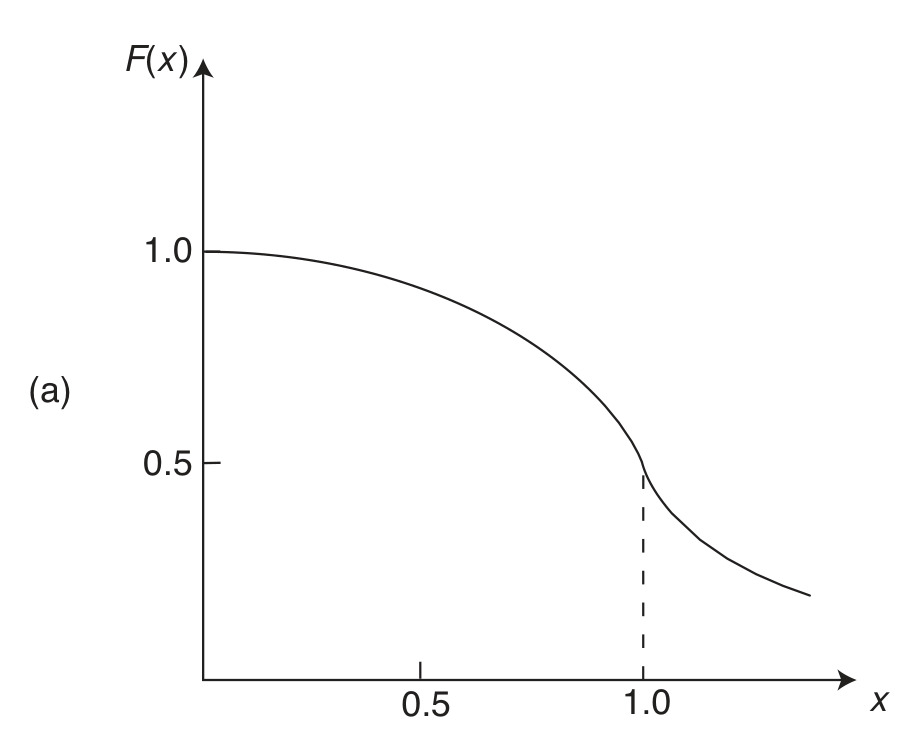
\includegraphics[width=0.55\textwidth]{figs/ch06/fig_6.1_a.jpg}\\[6pt]
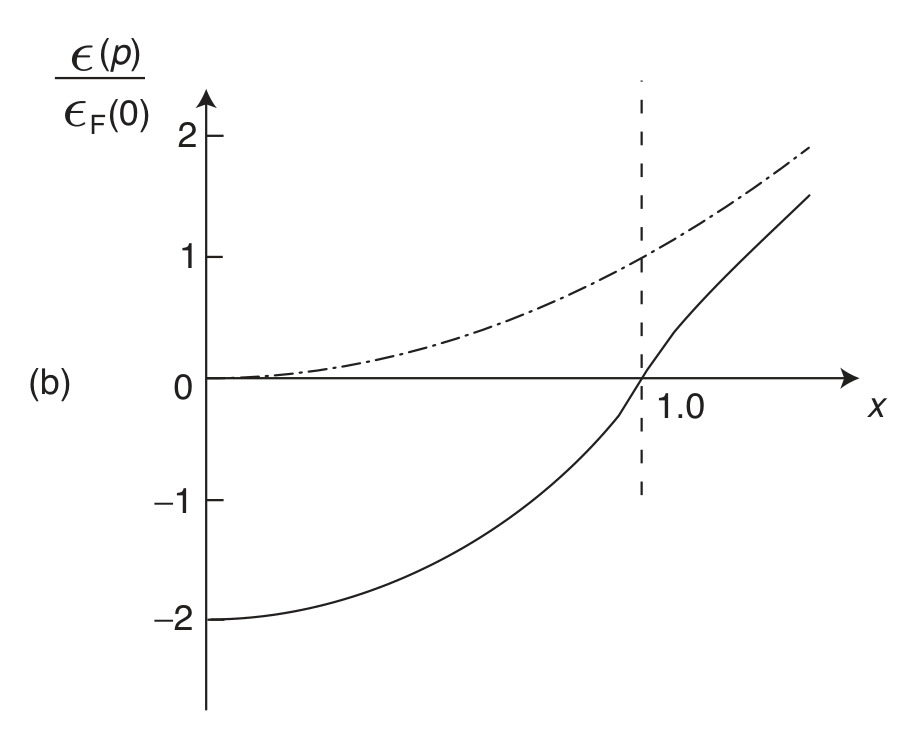
\includegraphics[width=0.55\textwidth]{figs/ch06/fig_6.1_b.jpg}
\caption*{图 6.1\quad (a) 由式 (6.16) 定义的函数$F(x)$在$r_{\mathrm{s}} = 3.0$下的图像。$F(x)$的斜率在$x \to 1$时发散，且$F(x = 1) = \frac{1}{2}$。对大的$x$，$F(x)$趋于$\frac{1}{3x^2}$。(b) 由式 (6.17) 定义的标度化哈特里–福克单粒子能量色散（实线）。哈特里–福克把带宽高估了一个附加常数$0.331\,r_{\mathrm{s}}\epsilon_{\mathrm{F}}^0$。带宽的这一增大完全来自交换相互作用。作为视觉引导，图中以点划线画出自由粒子的色散。}\label{fig:auto:6.1}
\end{figure}

哈特里–福克近似的另一困难是它高估了能量带宽，带宽定义为$\Delta = \epsilon(x = 1) - \epsilon(x = 0)$。对范围很广的金属而言，$\epsilon_{\mathrm{F}}^0$的无相互作用值很好地逼近实验观测到的带宽。在哈特里–福克层级，带宽扩大为
\begin{equation*}
\Delta = \epsilon_{\mathrm{F}}^0(1 + 0.331\,r_{\mathrm{s}}).
\tag{6.23}
\end{equation*}
带宽的增加$\sim 0.331\,r_{\mathrm{s}}$图示于图 6.1(b) 中。

\section{金属的内聚能}

哈特里–福克近似所应用的关键问题之一是金属的内聚能（cohesive energy）。把自由原子聚在一起形成金属时，原子的能量降低。内聚能定义为如下差值
\begin{equation*}
\epsilon_{\mathrm{coh}} = (\epsilon/\mathrm{atom})_{\mathrm{metal}} - (\epsilon/\mathrm{atom})_{\mathrm{free\ atom}},
\end{equation*}
在束缚的金属中它为负。碱金属中实测的内聚能为：

\begin{center}
表 6.1\\[4pt]
\begin{tabular}{lccccc}
\toprule
eV & Li & Na & K & Rb & Cs\\
\midrule
$\epsilon_{\mathrm{coh,expt}}$ & $-1.58$ & $-1.13$ & $-0.98$ & $-0.82$ & $-0.815$\\
\bottomrule
\end{tabular}
\end{center}

要定量计算内聚能，需要在哈特里–福克之外作两点改进。除了更好地描述电子间的关联之外，还必须超越离子构成均匀背景的近似，更精确地考虑电子与离子的相互作用以及离子的平均库仑能。我们此处遵循维格纳与塞茨（WS1933）计算金属内聚能的策略——正是这一方案使他们得以首次把量子力学定量地应用于计算固体的真实性质。

\subsection{维格纳–塞茨方法}

维格纳–塞茨方法的主要思想是把晶体划分为各含一个离子和$Z$个电子的（维格纳–塞茨）原胞，并对每个原胞内部的相互作用作相当准确的处理。由于每个原胞都是电中性的，原胞之间的相互作用能在第一级近似下可以忽略。内聚能于是由下式给出：
\begin{equation*}
\epsilon_{\mathrm{coh}} = \epsilon_0 - \epsilon_{\mathrm{atom}} + \epsilon_{\mathrm{kin}} + \epsilon_{\mathrm{coul}},
\tag{6.24}
\end{equation*}
其中$\epsilon_0$是原胞中传导电子的最低能量，物理上即导带底的能量；$\epsilon_{\mathrm{kin}}$是电子的平均动能；$\epsilon_{\mathrm{coul}}$是电子–电子的平均库仑能。

此时我们把注意力限于碱金属：每个原胞中只含一个传导电子和一个离子。起初可以忽略原胞内的电子–电子相互作用。最简单地把维格纳–塞茨原胞取为围绕离子的一个球。为计算$\epsilon_0$，我们在离子势存在下求解薛定谔方程
\begin{equation*}
\left(\frac{\hat{p}^2}{2m} + V_{\mathrm{ion}}\right)\varphi_0(\mathbf{r}) = \epsilon_0\varphi_0(\mathbf{r})
\tag{6.25}
\end{equation*}
以求最低的传导电子能级。每个原胞边界处的边界条件是法向导数$\varphi_0'(\mathbf{r}) = 0$。由此得到的各$\epsilon_0$值列于表 6.2。

\begin{center}
表 6.2\\[4pt]
\begin{tabular}{lccccc}
\toprule
eV & Li & Na & K & Rb & Cs\\
\midrule
$\epsilon_{\mathrm{atom}}$ & $-5.37$ & $-5.16$ & $-4.34$ & $-4.17$ & $-3.89$\\
$\epsilon_0$ & $-9.15$ & $-8.25$ & $-6.58$ & $-6.18$ & $-5.85$\\
$\epsilon_0 - \epsilon_{\mathrm{atom}}$ & $-3.78$ & $-3.09$ & $-2.24$ & $-2.01$ & $-1.95$\\
\bottomrule
\end{tabular}
\end{center}

显然，$\epsilon_0 - \epsilon_{\mathrm{atom}} < 0$，这源于晶体中相邻离子间的相互作用使电子离域化，从而最终降低了电子的能量。

对$\epsilon_0$最简单的估计假定离子提供一个中心的$1/r$势，并且由于与芯电子之间的不相容原理，电子到中心势的距离不能小于$a_0$。于是
\begin{equation*}
\epsilon_0 \simeq -n_{\mathrm{e}}\int_{a_0}^{r_{\mathrm{e}}} \mathrm{d}\mathbf{r}\,\frac{e^2}{r}
\tag{6.26}
\end{equation*}
\begin{equation*}
= -\frac{3e^2}{2r_{\mathrm{e}}^3}\left(r_{\mathrm{e}}^2 - a_0^2\right) = -\frac{40.82\,\mathrm{eV}}{r_{\mathrm{s}}}\left(1 - \frac{1}{r_{\mathrm{s}}^2}\right).
\tag{6.27}
\end{equation*}

接下来我们把传导电子的动能包括进来。自由气体中每个电子的动能由下式给出：
\begin{equation*}
\epsilon_{\mathrm{kin}}^0 = \frac{3}{5}\frac{p_{\mathrm{F}}^2}{2m} = \frac{2.21}{r_{\mathrm{s}}^2}\,\mathrm{Ry}.
\tag{6.28}
\end{equation*}
下面列出碱金属的$r_{\mathrm{s}}$值及相应的动能：

\begin{center}
表 6.3\\[4pt]
\begin{tabular}{lccccc}
\toprule
eV & Li & Na & K & Rb & Cs\\
\midrule
$r_{\mathrm{s}}$ & $3.22$ & $3.96$ & $4.87$ & $5.18$ & $5.57$\\
$\epsilon_{\mathrm{kin}}$ & $2.90$ & $1.92$ & $1.26$ & $1.12$ & $0.97$\\
\bottomrule
\end{tabular}
\end{center}

为定出量级，我们忽略库仑相互作用，仅由$\epsilon_0$（式 (6.27)）和动能按$\epsilon_{\mathrm{coh}} \approx \epsilon_0 - \epsilon_{\mathrm{atom}} + \epsilon_{\mathrm{kin}}$计算内聚能，得到：

\begin{center}
表 6.4\\[4pt]
\begin{tabular}{lccccc}
\toprule
eV & Li & Na & K & Rb & Cs\\
\midrule
$\epsilon_{\mathrm{coh,NI}}$ & $-0.89$ & $-1.17$ & $-0.97$ & $-0.89$ & $-0.98$\\
$\epsilon_{\mathrm{coh,expt}}$ & $-1.58$ & $-1.13$ & $-0.98$ & $-0.82$ & $-0.815$\\
\bottomrule
\end{tabular}
\end{center}

显然，这一层级的理论对内聚能的估计与实验的符合程度从尚可到很差。

现在我们把直接库仑能包括进来：把电子密度当作均匀的，并把每个原胞换成半径为$r_{\mathrm{e}}$的球。在这样的球中，半径$r < r_{\mathrm{e}}$的球内所包围的电子数为$n(r) = 4\pi r^3 n_{\mathrm{e}}/3$。直接库仑能为
\begin{equation*}
\epsilon_{\mathrm{direct}} = \int_0^{r_{\mathrm{e}}} \mathrm{d}\mathbf{r}\,\frac{e^2}{r}n_{\mathrm{e}}n(r).
\tag{6.29}
\end{equation*}
算出积分，我们得到
\begin{equation*}
\epsilon_{\mathrm{direct}} = \frac{3}{5}\frac{e^2}{r_{\mathrm{e}}} = \frac{6}{5r_{\mathrm{s}}}\,\mathrm{Ry}.
\tag{6.30}
\end{equation*}
中性维格纳–塞茨原胞之间的相互作用能是更高阶的修正，可以在更精确的计算中计入。

接着我们在哈特里–福克层级计入交换库仑能，仍假定电子密度均匀。由式 (6.15)，交换能为
\begin{equation*}
\epsilon_{\mathrm{exch}} = -\frac{0.916}{r_{\mathrm{s}}}\,\mathrm{Ry}.
\tag{6.31}
\end{equation*}
总的电子–电子库仑能于是为
\begin{equation*}
\epsilon_{\mathrm{coul}} = \epsilon_{\mathrm{exch}} + \epsilon_{\mathrm{direct}} = \frac{0.284}{r_{\mathrm{s}}}\,\mathrm{Ry},
\tag{6.32}
\end{equation*}
而内聚能变为
\begin{equation*}
\epsilon_{\mathrm{coh,HF}} = \epsilon_0 - \epsilon_{\mathrm{atom}} + \epsilon_{\mathrm{kin}} + \epsilon_{\mathrm{coul}}.
\tag{6.33}
\end{equation*}
库仑能以及新的内聚能与实验值（P1955）的比较如下所示：

\begin{center}
表 6.5\\[4pt]
\begin{tabular}{lccccc}
\toprule
eV & Li & Na & K & Rb & Cs\\
\midrule
$\epsilon_{\mathrm{coul}}$ & $1.24$ & $1.01$ & $0.82$ & $0.77$ & $0.72$\\
$\epsilon_{\mathrm{coh,HF}}$ & $0.32$ & $-0.16$ & $-0.15$ & $-0.12$ & $-0.26$\\
$\epsilon_{\mathrm{coh,expt}}$ & $-1.58$ & $-1.13$ & $-0.98$ & $-0.82$ & $-0.82$\\
\bottomrule
\end{tabular}
\end{center}

\begin{figure}[H]\centering
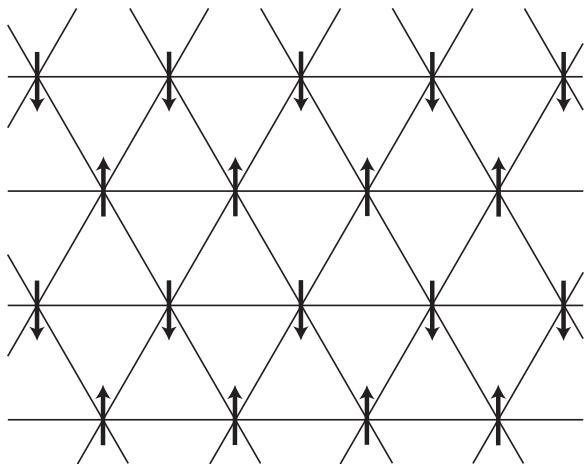
\includegraphics[width=0.5\textwidth]{figs/ch06/fig_6.2.jpg}
\caption*{图 6.2\quad 电子的二维（2d）维格纳晶格。当$d = 2$时，三角晶格使电子之间的$1/r$库仑排斥最小。每个格点上的箭头反映电子自旋的取向。由于三角晶格不是二分的（bipartite），即它无法被分成两个等价的子晶格，它不支持长程反铁磁序。蒙特卡罗计算（TC1989）表明，当$r_{\mathrm{s}} > 37$时，会发生向维格纳固体的转变，自旋组态如图所示。维格纳固体的形成已在液氦表面的电子（G1979）以及限制在GaAs与AlGaAs界面处运动的稀薄空穴气体（Y1999）中观察到。在外磁场存在时，维格纳晶体在更高密度下也应当稳定，因为磁场倾向于冻结电子的零点运动。在强垂直磁场下稀薄二维电子气上的实验（S1992）也证实了维格纳晶体的形成。}\label{fig:auto:6.2}
\end{figure}

显然，虽然哈特里–福克近似预言金属中的原子是束缚的，但它给不出准确的定量预言。事实上，无相互作用的图像$\epsilon_{\mathrm{coh,NI}}$反而好得多。为改进理论，我们需要计入更高阶的电子–电子相互作用，也就是说，需要更精确地确定关联对多体系统能量的影响。

\subsection{维格纳固体}

维格纳的插值方案（W1934）——在高密度（$r_{\mathrm{s}} \to 0$）端用微扰论处理系统，在低密度（$r_{\mathrm{s}} \to \infty$）端把它当作固体——更直接适用于计算关联对电子气能量的影响。维格纳的关键观察是：在均匀离子背景中的低密度电子气里，电子应当形成有序排列。维格纳晶体的二维类似物绘于图 6.2。基本思想是：在这一极限下，基态能量作为动能项与库仑项之和，由库仑排斥主导，因为$\epsilon_{\mathrm{kin}} \sim 1/r_{\mathrm{s}}^2$而$\epsilon_{\mathrm{coul}} \sim 1/r_{\mathrm{s}}$，故当$r_{\mathrm{s}} \to \infty$时$\epsilon_{\mathrm{kin}} < \epsilon_{\mathrm{coul}}$。为使库仑排斥极小，电子发现在能量上有利于把自己组织成有序排列。在三维情形，最有利的排列是体心立方（bcc）晶格，尽管面心排列在能量上与之相当接近；简单立方排列则较为不利。反铁磁的bcc晶格在$r_{\mathrm{s}} > 93$时稳定（CA1999）。向铁磁体的转变（OHB1999）似乎发生在$r_{\mathrm{s}} \approx 65$附近。

维格纳固体的能量完全由库仑能决定。为估计这一能量，我们计算一个中性维格纳–塞茨原胞的能量，这次原胞中心含有一个电子，四周是均匀的离子背景。如前所述，中性维格纳–塞茨原胞之间的相互作用能是高阶修正。在球形原胞中，均匀正背景与局域于中心的电子之间的相互作用能由下式给出：
\begin{equation*}
\epsilon_{\mathrm{ei}} \approx -n_{\mathrm{e}}e^2\int_0^{r_{\mathrm{e}}} \frac{\mathrm{d}\mathbf{r}}{r} = -\frac{3}{2}\frac{e^2}{r_{\mathrm{e}}}.
\tag{6.34}
\end{equation*}
补偿性的正背景提供一个均匀的静电能，它是前面讨论维格纳–塞茨方法时确定的直接库仑相互作用（式 (6.30)）$\epsilon_{\mathrm{direct}} \simeq 3e^2/5r_{\mathrm{e}}$的类似物。维格纳固体的能量于是为
\begin{equation*}
\epsilon_{\mathrm{WS}} = \left(\frac{3}{5} - \frac{3}{2}\right)\frac{e^2}{r_{\mathrm{e}}} = -\frac{9}{10}\frac{e^2}{r_{\mathrm{e}}} = -\frac{1.8}{r_{\mathrm{s}}}\,\mathrm{Ry}.
\tag{6.35}
\end{equation*}
电子绕其平衡位置的零点涨落对维格纳晶体能量的贡献按$1/r_{\mathrm{s}}^{3/2}$衰减（习题 6.5），在提取关联能的第一级近似时无需计入。

为辨认维格纳固体中的关联能，我们写出
\begin{equation*}
\epsilon_{\mathrm{WS}} = \epsilon_{\mathrm{exch}} + \epsilon_{\mathrm{corr}} = \left(\frac{-0.916}{r_{\mathrm{s}}} - \frac{0.884}{r_{\mathrm{s}}}\right)\mathrm{Ry}.
\tag{6.36}
\end{equation*}
对大的$r_{\mathrm{s}}$，关联能因而为
\begin{equation*}
\epsilon_{\mathrm{corr}} \approx -\frac{0.884}{r_{\mathrm{s}}}\,\mathrm{Ry},\quad r_{\mathrm{s}} \to \infty.
\tag{6.37}
\end{equation*}

在高密度区间，可以求助于盖尔曼（Gell-Mann）与布吕克纳（Brueckner）的微扰处理（GB1957）。在微扰论中，电子–电子相互作用的二阶项具有形式
\begin{equation*}
E_{\mathrm{coul}}^{(2)} = \sum_{\mu \neq 0} \frac{\langle p|V_{\mathrm{ee}}|\mu\rangle\langle\mu|V_{\mathrm{ee}}|0\rangle}{E_0 - E_\mu},
\tag{6.38}
\end{equation*}
其中$|\mu\rangle$是一个中间激发态。微扰展开中的所有项都可以用图形表示，这可以借维克（Wick）定理证明。所出现的二阶图形如图 6.3 所示。

\begin{figure}[H]\centering
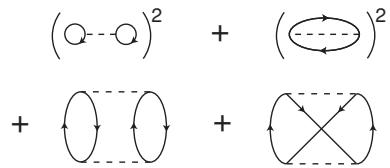
\includegraphics[width=0.6\textwidth]{figs/ch06/fig_6.3.jpg}
\caption*{图 6.3\quad 均匀电子气基态能量微扰展开中的二阶关联图形。实线表示电子，虚线表示两体库仑相互作用。}\label{fig:auto:6.3}
\end{figure}

图 6.3 中最后一个图形——只含单个电子回路的交换项——是对数发散的。盖尔曼与布吕克纳（GB1957）认识到，通过对整整一类这样的发散项作巧妙的重求和，可以得到一个有限但非解析的结果。的确，他们找到了电子气能量的一个展开式
\begin{equation*}
\epsilon_{\mathrm{GB}} = \left(\frac{2.21}{r_{\mathrm{s}}^2} - \frac{0.916}{r_{\mathrm{s}}} + 0.062\ln r_{\mathrm{s}} - 0.096 + \cdots\right)\mathrm{Ry}.
\tag{6.39}
\end{equation*}
注意非解析项$\ln r_{\mathrm{s}}$的出现。这一项反映出如下事实：系统的能量在$e^2 = 0$附近不可能关于$e^2$解析；事实上，$e^2 < 0$的电子系统的物理是自引力束缚云团的物理，与$e^2 > 0$的情形有质的不同。应用微扰论（即使在其重求和的形式下）的问题在于，真实金属位于$r_{\mathrm{s}} > 1$的区域，因此要得到定量准确的结果，就必须对整个级数求和。习惯上把电子系统的能量写成
\begin{equation*}
\epsilon = \epsilon_{\mathrm{kin}} + \epsilon_{\mathrm{exch}} + \epsilon_{\mathrm{corr}};
\tag{6.40}
\end{equation*}
的形式，以此定义关联能（correlation energy）；于是盖尔曼与布吕克纳关于高密度极限下关联能的结果为
\begin{equation*}
\epsilon_{\mathrm{corr}} \approx 0.062\ln r_{\mathrm{s}} - 0.096,\quad r_{\mathrm{s}} \to 0.
\tag{6.41}
\end{equation*}

取$r_{\mathrm{s}} = 1$处$\epsilon_{\mathrm{corr}} = -0.096\,\mathrm{Ry}$，我们可以本着维格纳的精神，在高密度与低密度结果之间写下一个简单的近似插值：
\begin{equation*}
\epsilon_{\mathrm{corr}} = -\frac{0.884}{r_{\mathrm{s}} + 8.21}\,\mathrm{Ry} = -\frac{12.03}{r_{\mathrm{s}} + 8.21}\,\mathrm{eV}.
\tag{6.42}
\end{equation*}
正如Pines（P1955）所指出的，$r_{\mathrm{s}} = 1$处的关联能更接近$-0.11\,\mathrm{Ry}$。尽管如此，我们仍在微扰方案（GB1957）的框架内工作，采用式 (6.42) 作为关联能的插值公式。利用式 (6.42)，我们得到关联能与内聚能：

\begin{center}
表 6.6\\[4pt]
\begin{tabular}{lccccc}
\toprule
eV & Li & Na & K & Rb & Cs\\
\midrule
$\epsilon_{\mathrm{corr}}$ & $-0.7$ & $-1.15$ & $-1.07$ & $-1.02$ & $-1.17$\\
$\epsilon_{\mathrm{coh,W}}$ & $-1.64$ & $-1.15$ & $-1.02$ & $-0.96$ & $-0.92$\\
$\epsilon_{\mathrm{coh,expt}}$ & $-1.58$ & $-1.13$ & $-0.98$ & $-0.82$ & $-0.815$\\
\bottomrule
\end{tabular}
\end{center}

使用维格纳插值所带来的改进是显著的。

然而，虽然式 (6.42) 是内聚能的一个有用插值公式，维格纳方案却隐含地假定：在稠密的微扰极限与晶体区间之间不会出现电子气的新相。这一假定其实毫无根据。事实上，固体物理中尚未解决的问题之一就是：维格纳晶体熔化时会出现什么样的物相。由于在维格纳熔化边界处无法使用微扰论，这个问题没有容易的解答。在本章撰写之时，对稀薄二维电子气的实验（K1999）表明这一相是奇异的。

\section*{小结}
\addcontentsline{toc}{section}{小结}

本章我们展示了如何在补偿性正背景中的电子气框架下实施哈特里–福克程序。关键结果是：本征函数为平面波，但单粒子能级因交换相互作用而降低。交换相互作用使每个电子周围的电子密度减小。然而，哈特里–福克描述不能准确给出带宽或比热，后者呈$T/\ln T$的行为。在第9章中，我们将展示引入电子屏蔽如何弥补哈特里–福克的某些失败之处。为准确估计晶体的内聚能，维格纳插值方案相当成功。该方案背后的物理是：在足够低的密度下，有序的电子晶格使电子气的能量极小。在$d = 3$时体心立方晶格占优，而在$d = 2$时形成电子的三角晶格。

\section*{习题}
\addcontentsline{toc}{section}{习题}

\textbf{习题 6.1}\quad 证明：
\begin{equation*}
\frac{1}{2}\int_0^{p_{\mathrm{F}}} \epsilon_{\mathrm{exch}}(\mathbf{p})\frac{\mathrm{d}\mathbf{p}}{(2\pi\hbar)^3} = -\frac{e^2 p_{\mathrm{F}}^4}{4\pi^3\hbar^4}.
\end{equation*}

\textbf{习题 6.2}\quad 假定电子气比热具有哈特里–福克表达式$\sim T/|\ln T|$，试确定Na在什么温度以下对线性比热的修正会变得显著（比如说10\%）。

\textbf{习题 6.3}\quad 考虑一个通过形如$V(r) = V_0\mathrm{e}^{-r/a}/r$的势相互作用的均匀电子气。(a) 对该系统求解哈特里–福克方程，求出本征函数与激发谱$\epsilon(\mathbf{p})$，并计算费米能量$\epsilon_{\mathrm{F}} = \mu$。(b) 在哈特里–福克层级，证明有效质量$m^*$完全由交换贡献决定。在$k_{\mathrm{F}}a \ll 1$和$k_{\mathrm{F}}a \gg 1$两个极限下显式计算$m^*$。(c) 证明当$k_{\mathrm{F}}a \gg 1$时，交换相互作用对$\epsilon_{\mathrm{F}}$的贡献可以忽略，而对$k_{\mathrm{F}}a \ll 1$的短程相互作用，直接项与交换项相当。

\textbf{习题 6.4}\quad 用如下变分计算估计维格纳–塞茨原胞中电子的最低能量$\epsilon_0$。假定离子产生的势在$r > r_{\mathrm{c}}$时为库仑势，在$r \le r_{\mathrm{c}}$时为排斥性硬核，其中$r_{\mathrm{c}}$是离子芯中最外层被占据玻尔轨道的半径。取试探波函数为只感受硬核排斥、不感受库仑吸引的电子的正确基态（连同边界条件在内）。将结果用eV表示，并与更精细的结果比较。

\textbf{习题 6.5}\quad 假设原胞为球形，试确定维格纳晶格中的电子偏离其平衡位置时所感受的势。计算电子在此势中的零点能，并证明低密度电子气能量的第一阶修正为每电子$3/r_{\mathrm{s}}^{3/2}\,\mathrm{Ry}$。

\textbf{习题 6.6}\quad 处于正电荷补偿背景中的二维电子气表现出净磁化强度，即上下自旋布居数之差。电子通过$1/r$相互作用。定义电子气中的相对磁化强度为
\begin{equation*}
\xi = \frac{n_\uparrow - n_\downarrow}{n_\uparrow + n_\downarrow}.
\tag{6.43}
\end{equation*}
先证明上下自旋的费米动量可以写为
\begin{equation*}
p_{\mathrm{F}\uparrow} = p_{\mathrm{F}}\sqrt{1 + \xi},\qquad p_{\mathrm{F}\downarrow} = p_{\mathrm{F}}\sqrt{1 - \xi}.
\tag{6.44}
\end{equation*}
在哈特里–福克层级，计算电子气的基态能量作为$\xi$的函数。对哪些$\xi$值基态是稳定的？估计完全极化（铁磁）电子气的基态能量低于完全未极化（$\xi = 0$）气体的$r_{\mathrm{s}}$值。

\section*{参考文献}
\addcontentsline{toc}{section}{参考文献}

\begin{itemize}[leftmargin=2em,itemsep=0pt,parsep=0pt,label={}]
\item [B1936] J. Bardeen, Phys. Rev. 50, 1098 (1936); see also E. P. Wohlfarth, Phil. Mag. 41, 534 (1950).
\item [CA1999] D. M. Ceperley and B. J. Alder, Phys. Rev. Lett. 45, 566 (1980); see also D. Ceperley, Nature (London) 397, 386 (1999).
\item [GB1957] M. Gell-Mann and K. A. Brueckner, Phys. Rev. 106, 364 (1957).
\item [G1979] C. C. Grimes and G. Adams, Phys. Rev. Lett. 42, 795 (1979).
\item [K1999] S. V. Kravchenko, D. Simonian, M. P. Sarachik, W. Mason, and J. E. Furneaux, Phys. Rev. Lett. 77, 4938 (1996).
\item [OHB1999] G. Ortiz, M. Harris, and P. Ballone, Phys. Rev. Lett. 82, 5317 (1999).
\item [P1955] D. Pines, Advances in Solid State Physics, eds. F. Seitz and D. Turnbull (Academic Press, New York, 1955), Vol. I, p. 373.
\item [S1992] M. B. Santos, Y. W. Suen, M. Shayegan, Y. P. Li, L. W. Engel, and D. C. Tsui, Phys. Rev. Lett. 68, 1188 (1992). For a theoretical prediction for the onset of a Wigner crystal in the quantum Hall regime, see P. K. Lam and S. M. Girvin, Phys. Rev. B 30, 473 (1984).
\item [TC1989] B. Tanatar and D. M. Ceperley, Phys. Rev. B 39, 5005 (1989).
\item [W1934] E. Wigner, Phys. Rev. 46, 1002 (1934).
\item [WS1933] E. Wigner and F. Seitz, Phys. Rev. 43, 804 (1933); 46, 509 (1933).
\item [Y1999] J. Yoon, C. C. Li, D. Shahar, D. C. Tsui, and M. Shayegan, Phys. Rev. Lett. 82, 1748 (1999).
\end{itemize}
